\section{CS 设计模式}

\subsection{模块分工}

\subsubsection{模块作用}

在网易的官方教程中,较为复杂的模组均采用了 CS 分离的设计模式,在我们模组中,改模式下三个模块负责:
\begin{itemize}
    \item Client: 负责客户端事件。
    \item Common: 负责模组数据操作。
    \item Server: 负责服务端事件。
\end{itemize}

这三个模块通过事件传递信息,其中 client 和 server 模块不可以相互 import。必须保证 CS 分离。但是他们都可以从 common 模块中获取数据。

本模组的 CS 设计模式中的三个主要模块分工如下:
\begin{itemize}
    \item Client 模块负责客户端事件的处理,Client 模块需要处理的事件较少,多为向服务端传递响应事件。在本模组中主要负责一些 UI 交互操作。
    \item Server 模块是主要逻辑模块,大部分逻辑均在 Server 模块中实现。此外,为了减少 Server 模块的负担,一些数据的预处理放在了 common 模块中实现。
    \item Common 模块主要存放数据,由于无法在脚本中读写 json 文件,数据多放在脚本文件中,以字典,列表的形式存储。
\end{itemize}

\subsubsection{模块之间交互}

Client 和 Server 模块都拥有 System 子模块(System 模块也代指 Client/Server 模块),这是这两个模块之间交互的唯一通道,即通过事件进行交互。其它子模块交互仅允许向 System 传递信息或者获取 System 进行操作。

原则上 Client 和 System 的任意模块都可以引用 Common 模块中的内容,但我们规定仅可调用 Common 中的 Facade 模块。一般地 Common 中的数据均为只读数据,也不会给出数据更改的接口。

模块之间交互的接口如下:
\begin{itemize}
    \item System: Client 和 System 之间通过 System 的事件进行交互。
    \item Facade: 提供 Common 模块的对外接口,Server 模块调用 Common 模块仅能从 Facade 中获取。
\end{itemize}

\newpage

\subsection{模块内部设计}

\subsubsection{Common 模块}

Common 模块是存储数据与对数据简单处理的模块,所有的常量,不可变数据均需放在这里,并且模块负责建立获取数据的接口。

在 Common 模块中有以下子主要模块\footnote{交互: 可以调用那些模块}:

\begin{table}[H]
    \centering
    \caption{Common 模块类设计}
    \label{table:Common 模块类设计}
    \setlength{\tabcolsep}{4mm}
    \begin{tabular}{l|l|lll}
        \toprule
        \textbf{子模块} & \textbf{角色} & \textbf{作用} & \textbf{独有} & \textbf{交互} \\
        \midrule
        data & 数据结构 & 存储数据 & \checkmark & - \\
        && \multicolumn{3}{l}{相当于 json 文件,用于保存数据。}  \\
        \midrule
        entity & 数据结构 & 将数据构造为类 & \checkmark & Config \\
        && \multicolumn{3}{l}{用户获取 data 模块中的数据并构造为对应的类}  \\
        \midrule
        proxy & 逻辑算法 & 对数据进行简单的逻辑处理。 & \checkmark & Factory/Utils \\
        && \multicolumn{3}{l}{提供对 entity 的部分操作功能,外部仅能从 proxy 对数据进行操作。}  \\
        \midrule
        factory & 逻辑算法 & 工厂类 &  & Manager/Entity \\
        && \multicolumn{3}{l}{统一由 Factory 创建类实例并进行管理。}  \\
        \midrule
        Facade & 对外接口 & 抽象工厂类,对外提供接口。 & \checkmark & Factory/Utils \\
        && \multicolumn{3}{l}{System 通过 Facade 和 Common 交互。}  \\
        \midrule
        utils & 逻辑算法 & 工具类,提供一些通用方法 & & - \\
        && \multicolumn{3}{l}{通用的工具类,一般只包含函数。}  \\
        \bottomrule
    \end{tabular}
\end{table}

特殊模块的说明:
\begin{itemize}
    \item \textbf{utils}: 不同系统可以使用同一个 utils 工具,而其它子模块,不同的系统间不可以交互。utils 通过 facade 提供外部接口。
    \item \textbf{proxy}: proxy 是数据代理类,将数据与对数据的操作解耦。proxy 不要直接访问 Entity,应该从 Factory 中获取 Entity 对象。
    \item \textbf{facade}: 注意 facade 是提供对外的接口,它仅起到一个统一外部接口的作用,内部模块间调用,应尽量使用 Factory 模块。
\end{itemize}

Common 模块内部交互关系如下:

\begin{figure}[H]
    \scriptsize
    \centering
    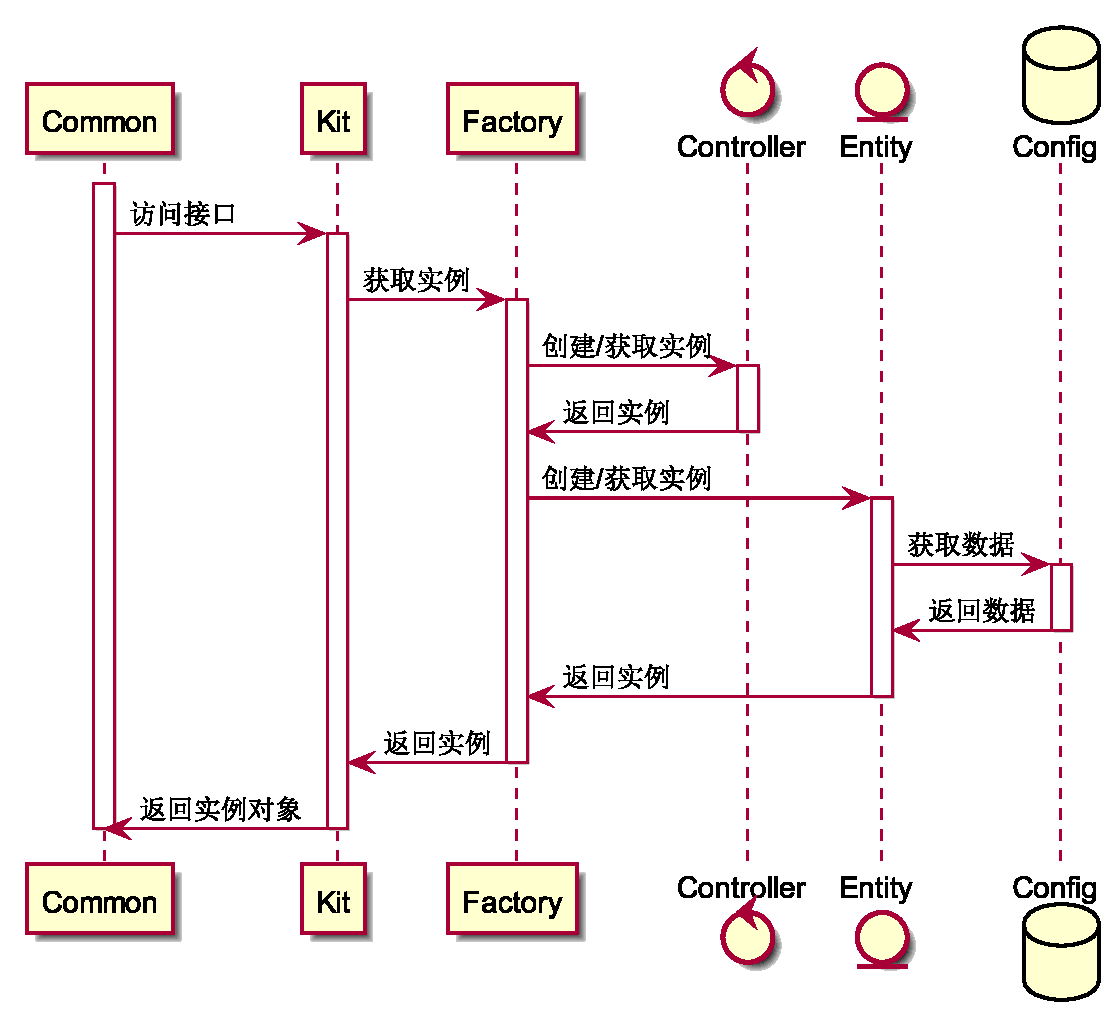
\includegraphics[width=10cm]{images/puml/common.eps} 
    \caption{Common 模块内部关系}
    \label{fig:Common 模块内部关系}
\end{figure}

Common 模块主要作用是向 System 模块提供数据与简单的数据操作;故采用类似 MVC 的结构进行管理。Common 模块内部交互方式如下:
\begin{itemize}
    \item facade: 提供外部接口,所有向 System 模块提供的接口都在此声明。
    \item factory: 提供内部接口,所有与数据相关的类与实例均由 factory 提供并进行管理。如果不涉及到数据(例如 utils 模块),无需经过 factory,由其他模块直接调用。
\end{itemize}

\subsubsection{System 模块}

Client/Server 负责处理客户端,服务端处理。它们的文件交互逻辑类似,故放在一起。他们有以下主要模块:

\begin{table}[H]
    \centering
    \caption{Client/Server 模块类设计}
    \label{table:Client/Server 模块类设计}
    \setlength{\tabcolsep}{4mm}
    \begin{tabular}{l|l|lll}
        \toprule
        \textbf{子模块} & \textbf{角色} & \textbf{作用} & \textbf{独有} & \textbf{交互} \\
        \midrule
        ui & 逻辑算法 & 负责 ui 构建与响应 & \checkmark & Utils \\
        && \multicolumn{3}{l}{管理与 ui 对应的 json 文件}  \\
        \midrule
        Manager & 逻辑算法 & 简单的逻辑处理与管理。 & \checkmark & Utils/Factory \\
        && \multicolumn{3}{l}{对客户端 ui/System 进行管理}  \\
        \midrule
        Factory & 逻辑算法 & 工厂类 &  & Manager/ui \\
        && \multicolumn{3}{l}{统一由 Factory 创建类实例并进行管理。}  \\
        \midrule
        Utils & 逻辑算法 & 工具类,提供一些通用方法 & & - \\
        && \multicolumn{3}{l}{通用的工具类,一般只包含函数。}  \\
        \midrule
        System & 接口/逻辑 & 系统,负责相互通信与基本的逻辑处理 & \checkmark & Factory/Utils \\
        && \multicolumn{3}{l}{最主要的类}  \\
        \bottomrule
    \end{tabular}
\end{table}

特殊模块说明:
\begin{itemize}
    \item \textbf{ui}: ui 相关的逻辑操作,仅在 Client 中出现。
    \item \textbf{Manager}: 与 Controller 不同,Manager 往往是一对多的关系,Client 的 Manager 通常仅有一个实例,而 Server 的 Manager 往往绑定在实体上,拥有多个实例。
    \item \textbf{事件}: Client 与 Server 之间通过事件相互传递数据,所以不需要创建 Kit 接口。
\end{itemize}

与 Common 模块不同的,System 模块并没有类似 MVC 的结构,所有子模块几乎都是为 System 模块服务的,可以理解为将 System 中的逻辑有规律地放入到了其它子模块中。

\subsection{模块接口}
\subsubsection{模块内部}

模块内部可以相互 import,模块也可以引用子模块中的内容,但子模块一般不允许访问父级模块中的内容,如需访问,应从 Factory 模块中获取。Factory 模块因此也负责管理类实例化的相关操作,必要情况下建立注册表。

\subsubsection{模块之间}
Common 模块通过 Kit 子模块向外提供接口,System(Client/Server) 模块通过事件交互信息。较为特殊的,如出现在 Client 的非 System 子模块中传递事件。需要获取系统实例节点,再传递事件。

\newpage